\renewcommand{\EntradaBibtex}{virtualworlds5040053}

\begin{frame}{\citetitle{\EntradaBibtex} \footnotemark[1] (1)}
Visualización de materiales híbridos multifuncionales
\begin{itemize}
\item Los materiales híbridos pueden integrar múltiples fases activas dentro de una misma estructura.
\item Su comportamiento depende de la interacción entre diferentes componentes.
\item Los diagramas 2D tradicionales dificultan comprender:
\begin{itemize}
  \item La distribución espacial de los componentes.
  \item La relación entre estructura y función.
  \item Los mecanismos de interacción.
\end{itemize}
\item Se propone utilizar visualización 3D interactiva y realidad aumentada (RA) para mejorar la comunicación científica, la cual permite explorar la estructura de un material complejo de una manera más intuitiva.
\end{itemize}
%La visualización inmersiva permite explorar la estructura de un material complejo de una manera más intuitiva que una representación estática.
\footnotetext[1]{\fullcite{\EntradaBibtex}}
\end{frame}

\begin{frame}{\citetitle{\EntradaBibtex} (2)}

Multifunctional Hybrid Material (MHM-App)

La aplicación representa una esfera multifuncional formada por:
\begin{itemize}
\item TiO$_2$: fase fotocatalítica.
\item Fe$_3$O$_4$ (magnetita): fase magnética.
\item Carbón activado: material adsorbente.
\item Clinoptilolita con hipoclorito: agente de liberación/control.
\item CuO: componente con función antimicrobiana.
\item Alginato de sodio: matriz encapsulante formada mediante gelación iónica.
\item Quitosano reticulado: recubrimiento externo.
\end{itemize}
La aplicación permite observar simultáneamente la estructura global y los diferentes materiales que la constituyen.
\end{frame}



\begin{frame}{\citetitle{\EntradaBibtex} (3)}

Aplicación móvil de visualización 3D + RA, proporciona dos modos complementarios:

\begin{columns}

% Column 1
\column{.4\linewidth}

\item Modo Realidad Aumentada
\begin{itemize}
\item Detecta una superficie horizontal.
\item Utiliza raycasting para colocar la esfera.
\item Permite observar el material integrado en el entorno real.
\end{itemize}

\column{.6\linewidth}
\begin{center}
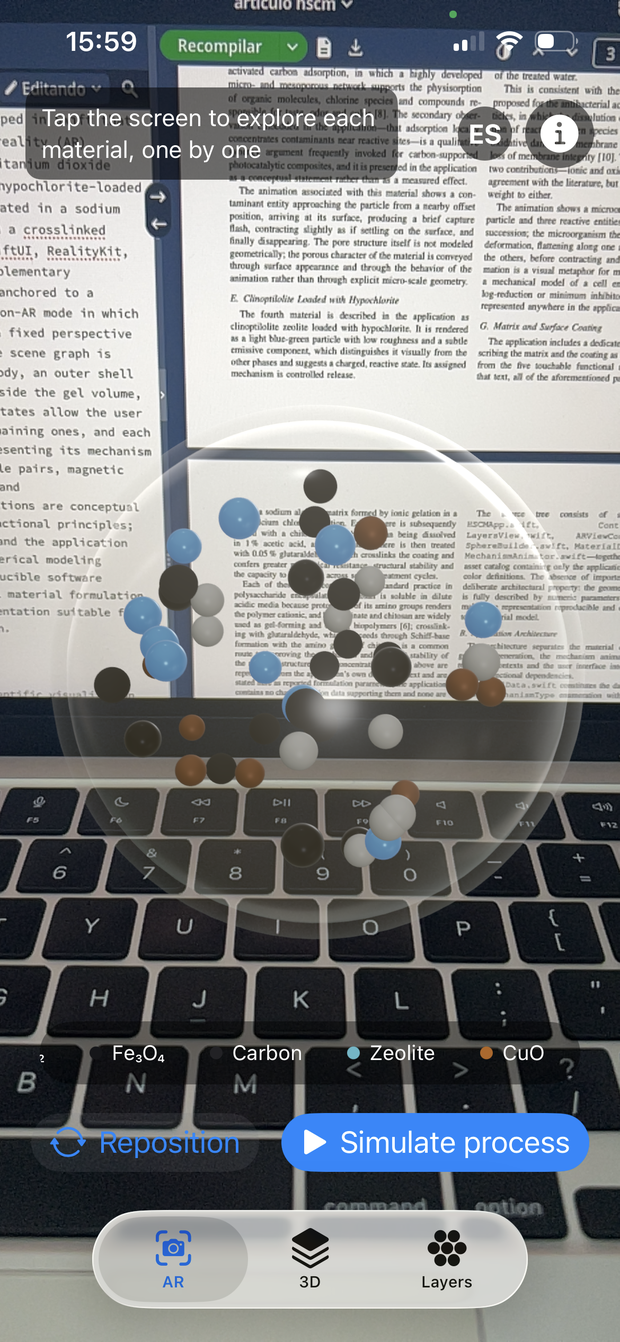
\includegraphics[width=0.20\linewidth]{2026_Augmented_Reality_Multifunctional_Hybrid_Materials/figs/hscm1_en.PNG}
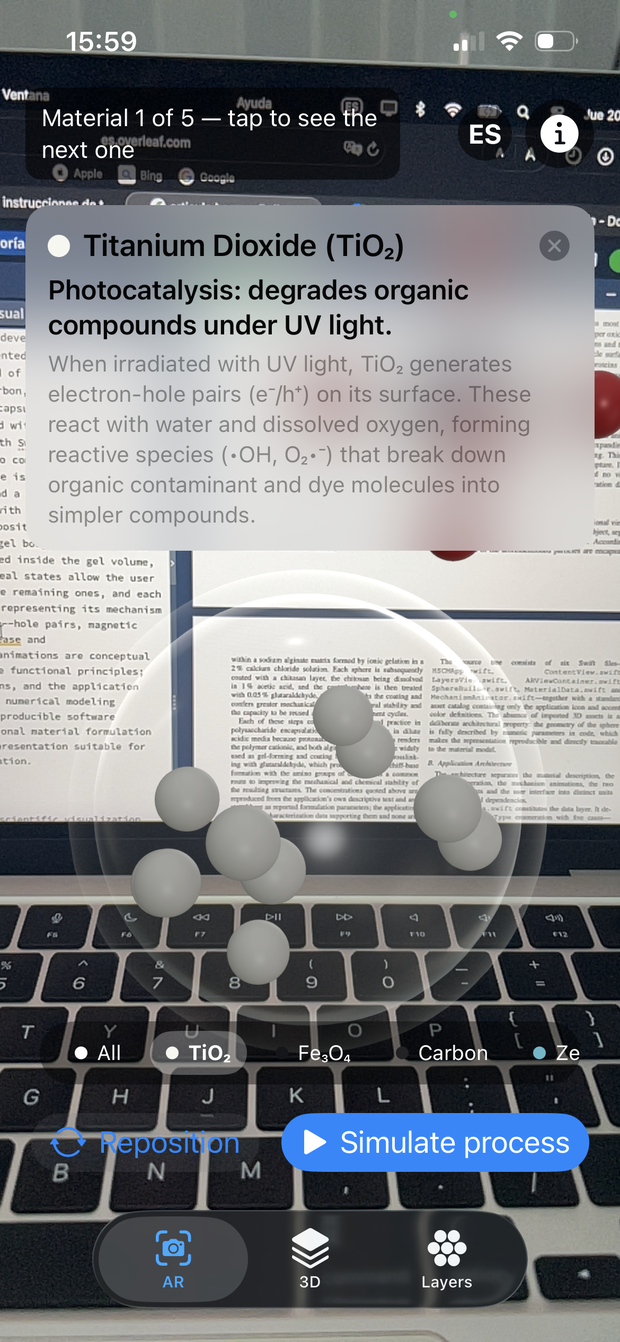
\includegraphics[width=0.20\linewidth]{2026_Augmented_Reality_Multifunctional_Hybrid_Materials/figs/hscm2_en.PNG}
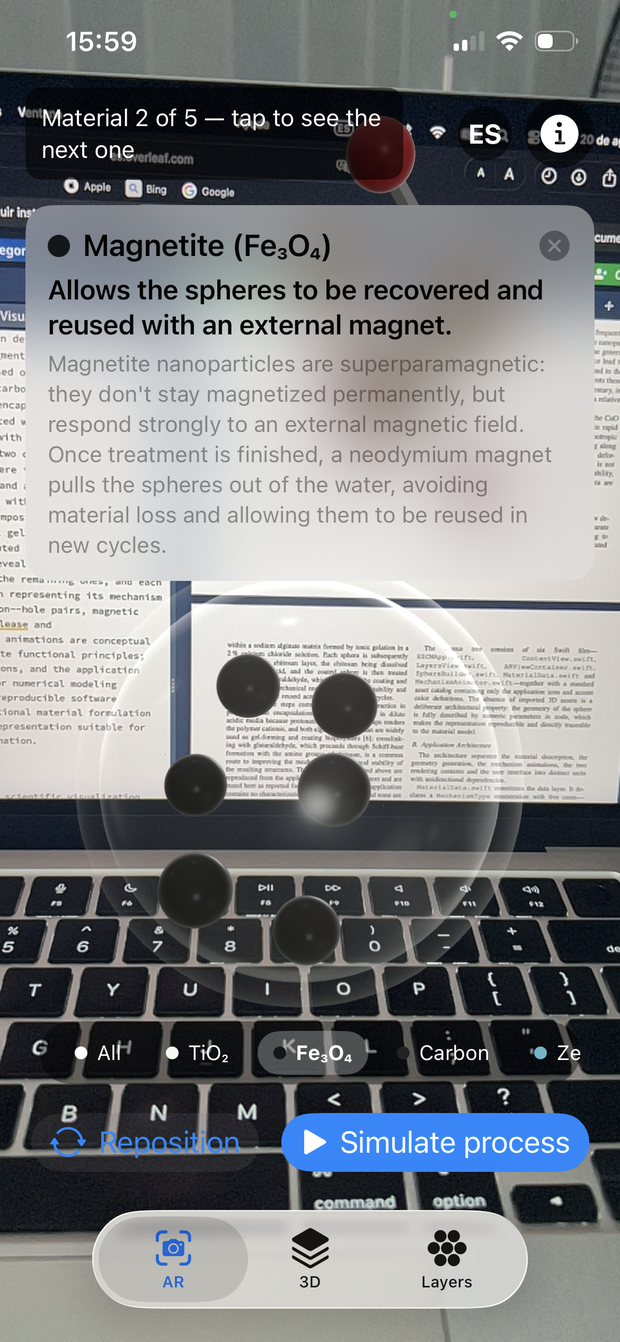
\includegraphics[width=0.20\linewidth]{2026_Augmented_Reality_Multifunctional_Hybrid_Materials/figs/hscm4_en.PNG}
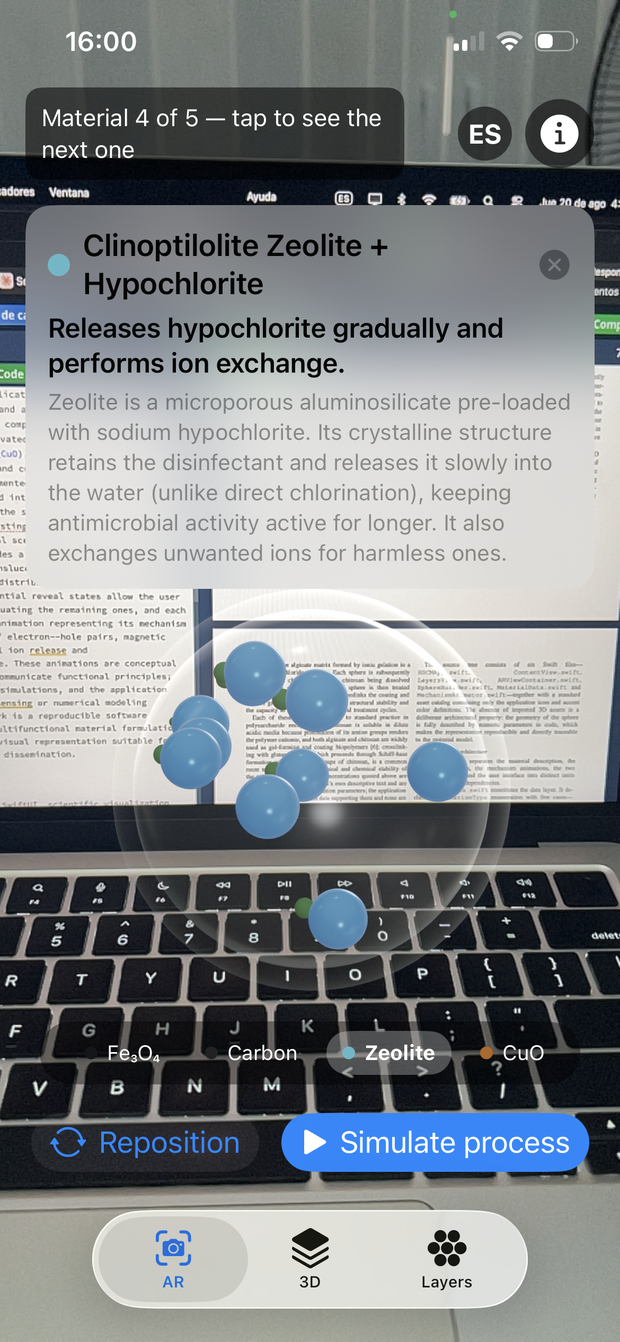
\includegraphics[width=0.20\linewidth]{2026_Augmented_Reality_Multifunctional_Hybrid_Materials/figs/hscm7_en.PNG}                                
\end{center}   
\end{columns}
\end{frame}


\begin{frame}{\citetitle{\EntradaBibtex} (4)}
\begin{columns}
% Column 1
\column{.4\linewidth}
Modo no-RA / entorno virtual
\begin{itemize}
\item La misma geometría 3D se presenta en una escena virtual.
\item Cámara con perspectiva fija.
\item Iluminación explícita para facilitar la inspección.
\end{itemize}
\column{.6\linewidth}
\begin{center}
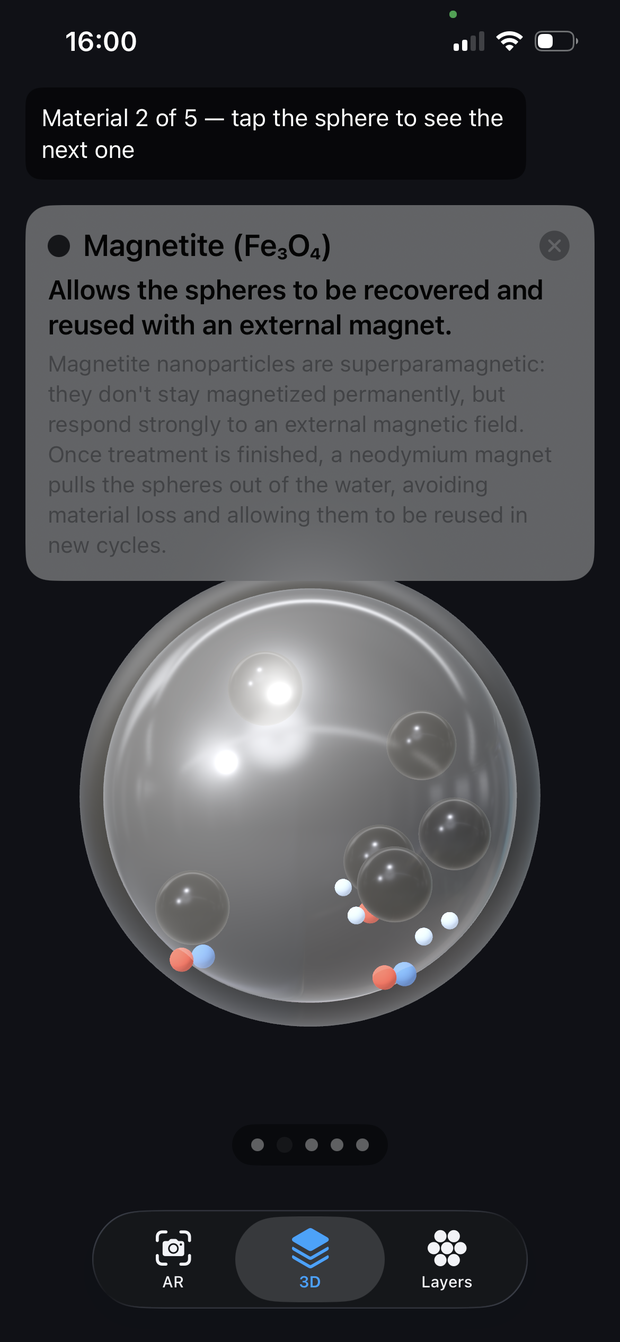
\includegraphics[width=0.20\linewidth]{2026_Augmented_Reality_Multifunctional_Hybrid_Materials/figs/hscm11_en.PNG}
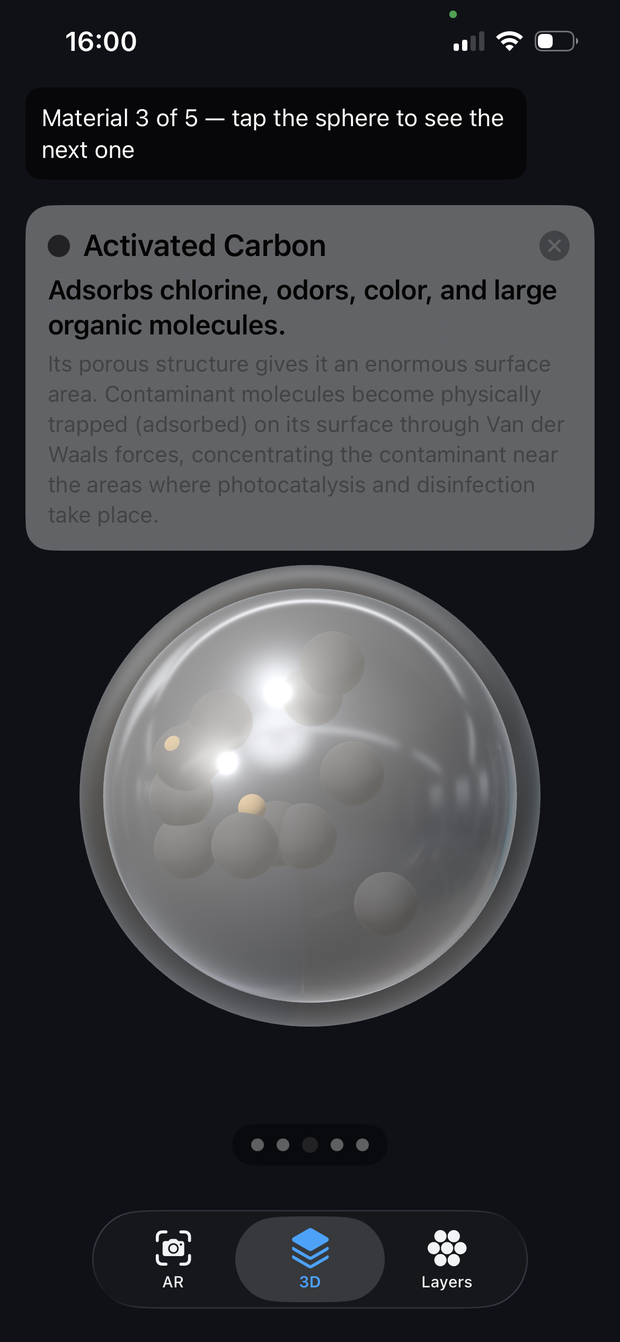
\includegraphics[width=0.20\linewidth]{2026_Augmented_Reality_Multifunctional_Hybrid_Materials/figs/hscm12_en.PNG}
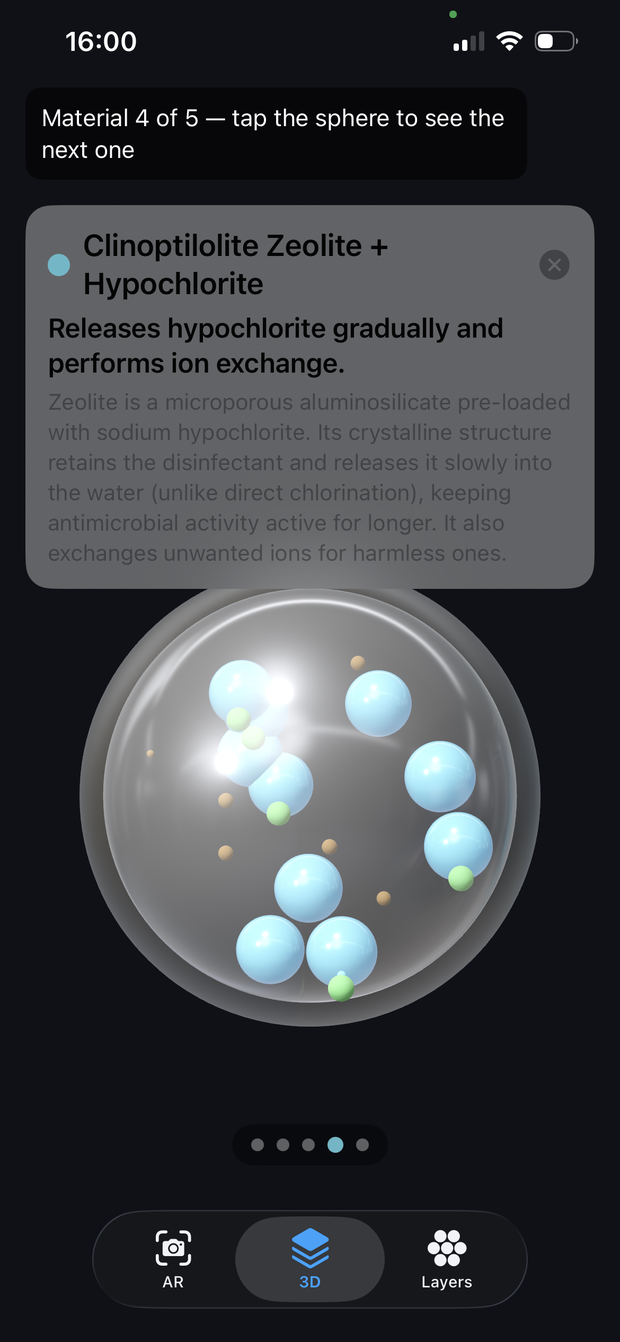
\includegraphics[width=0.20\linewidth]{2026_Augmented_Reality_Multifunctional_Hybrid_Materials/figs/hscm13_en.PNG}
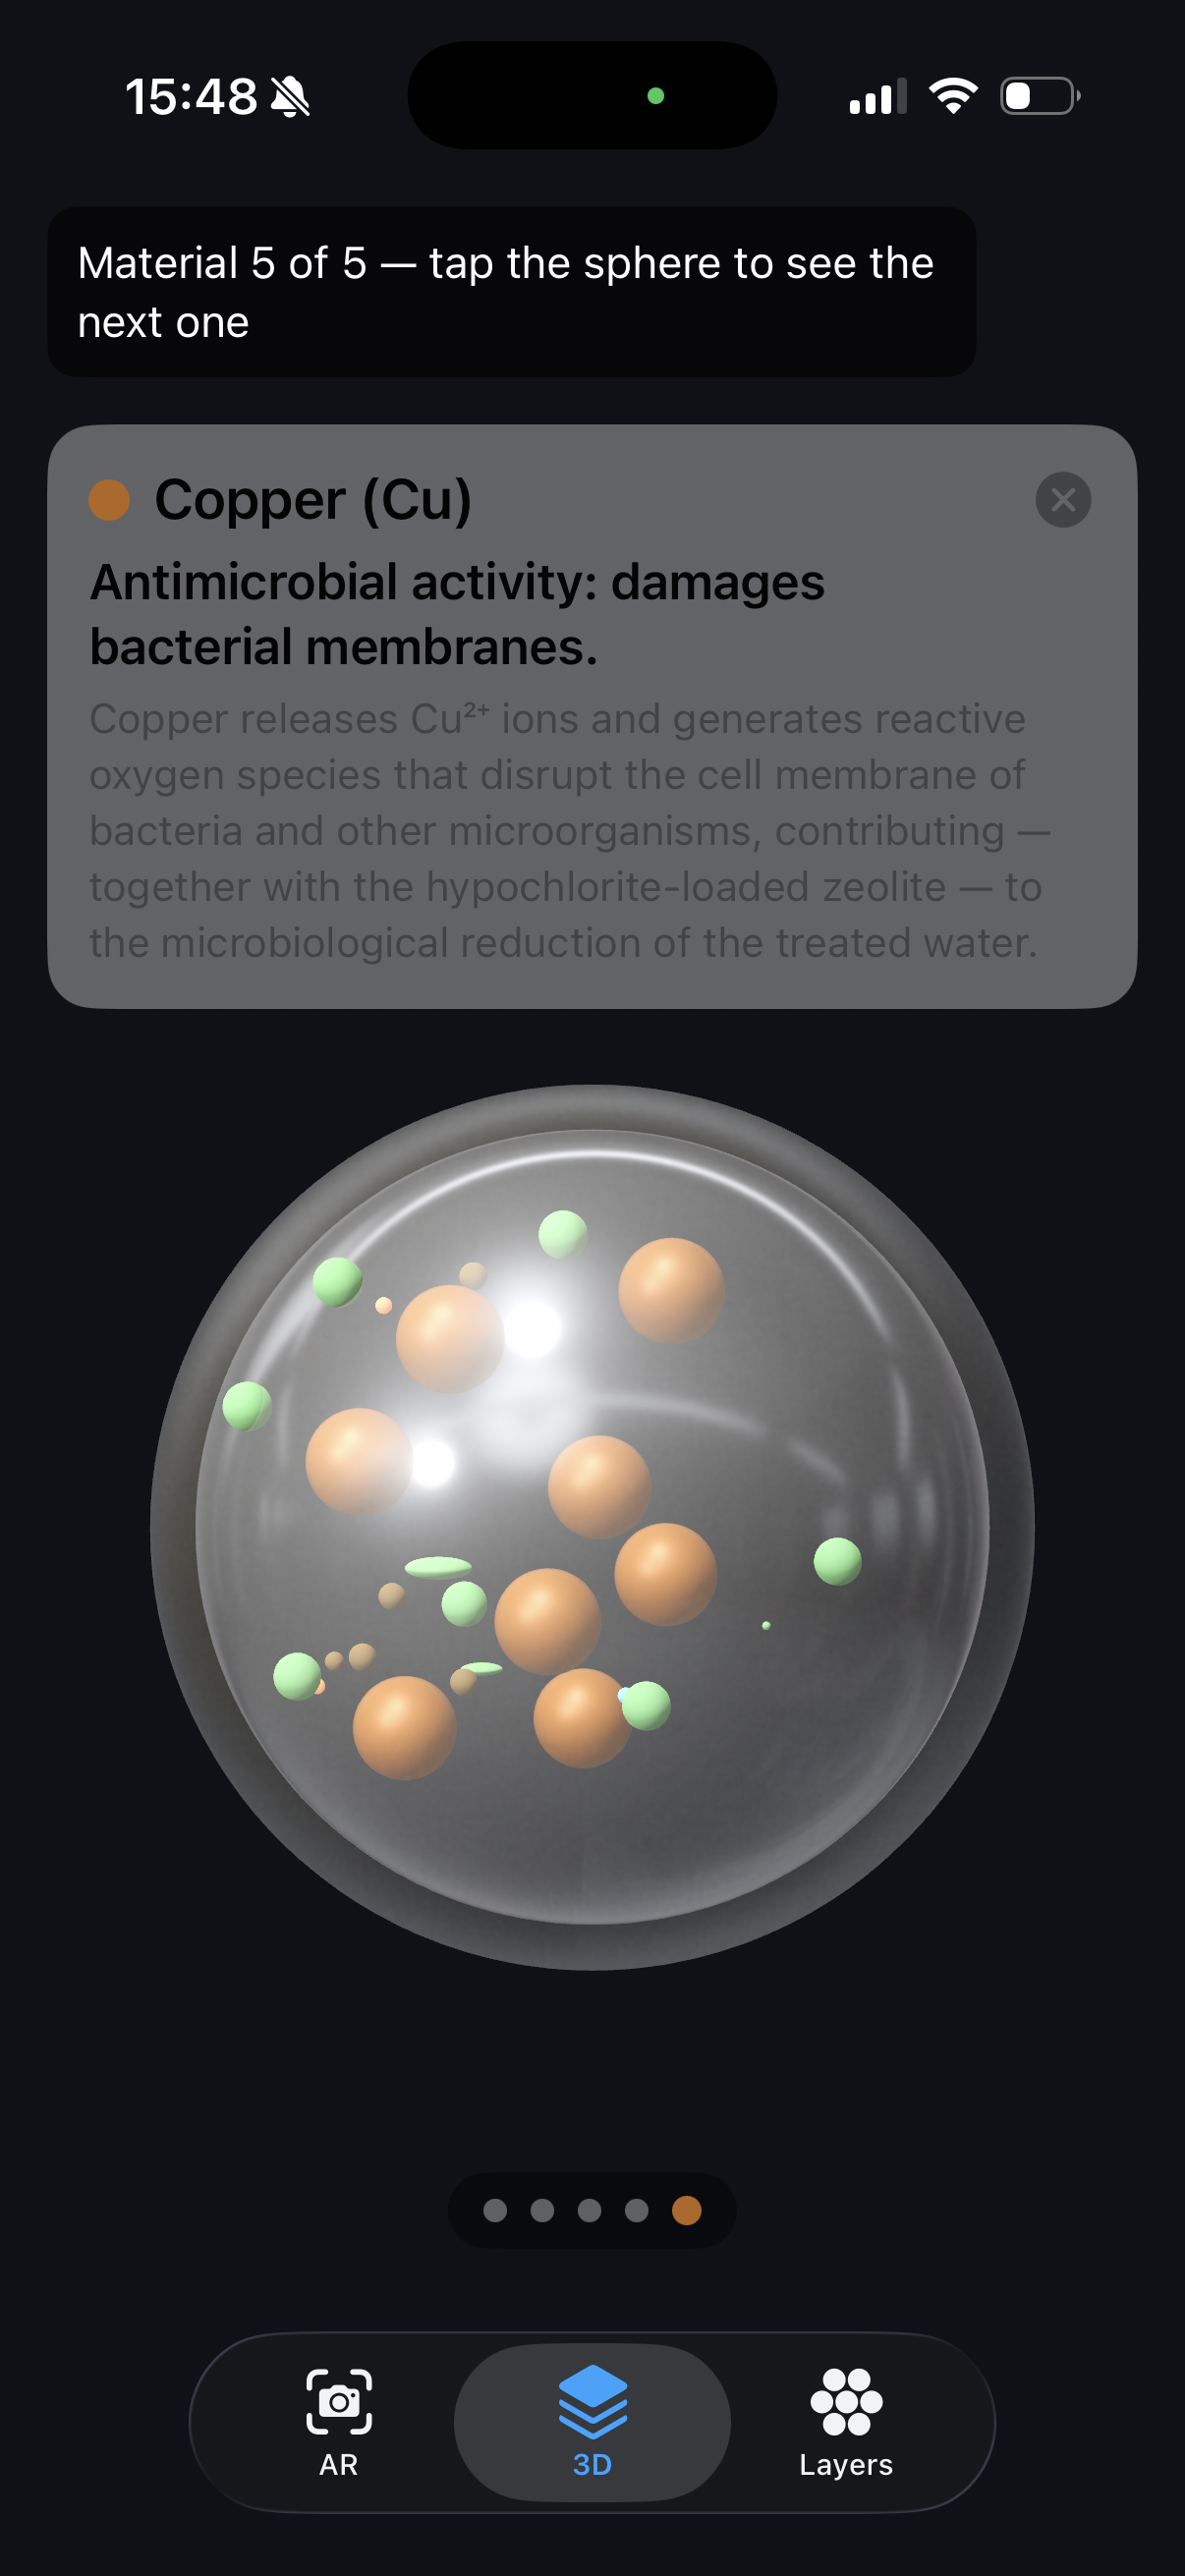
\includegraphics[width=0.20\linewidth]{2026_Augmented_Reality_Multifunctional_Hybrid_Materials/figs/hscm14_en_new.PNG}                                
\end{center}   
\end{columns}
\end{frame}


\begin{frame}{\citetitle{\EntradaBibtex} (5)}
Contribución principal
\begin{itemize}
\item Integración de RA + visualización 3D interactiva en una aplicación móvil.
\item Representación de la coexistencia espacial de múltiples fases dentro de un material híbrido.
\end{itemize}

Aplicaciones potenciales
\begin{itemize}
\item Educación: enseñanza de materiales y procesos químicos.
\item Comunicación científica: explicación de estructuras complejas.
\item Colaboración interdisciplinaria: interacción entre especialistas.
\item Ciencia de materiales: exploración de estructuras multifuncionales.
\end{itemize}
MHM-App demuestra el potencial de la RA y la visualización 3D móvil como herramientas para comprender, comunicar y explorar materiales multifuncionales complejos.
\end{frame}

